\documentclass[technicalreport]{ieicej}
\usepackage[dvipdfmx]{graphicx}
\usepackage[T1]{fontenc}
\usepackage{lmodern}
\usepackage{textcomp}
\usepackage{latexsym}
\usepackage{amsmath}
\usepackage{cite}
\usepackage{tikz}
\usepackage{geometry}
\usepackage{url}
\usepackage{schemabloc}
\usepackage{tikz}
\usepackage{makecell}
\usetikzlibrary{arrows}

\usetikzlibrary{positioning,fit,calc}
\tikzset{block/.style={draw, thick, text width=1cm, minimum height=0.5cm, align=center}, line/.style={-latex}}  

\renewcommand{\figurename}{Fig.} % name the picture Fig.num
\renewcommand{\tablename}{Table } % name the table Table num
\renewcommand{\refname}{REFERENCE} % insert reference 

%调整文件显示位置和纸张
\geometry{
	a4paper,
	total={170mm,257mm},
	left=20mm,
	top=20mm,
}

\hoffset=-5mm
\voffset=-5mm

\def\IEICEJcls{\texttt{ieicej.cls}}
\def\IEICEJver{3.0}
\newcommand{\AmSLaTeX}{%
$\mathcal A$\lower.4ex\hbox{$\!\mathcal M\!$}$\mathcal S$-\LaTeX}
\def\BibTeX{{\rmfamily B\kern-.05em{\scshape i\kern-.025em b}\kern-.08em
T\kern-.1667em\lower.7ex\hbox{E}\kern-.125em X}}

\jtitle{M1課題レポート 第3回}
\jsubtitle{}
\etitle{Technical Report for M1 Labwork 3rd}
\esubtitle{}
\authorlist{
\authorentry[liuyuchen@radio.ict.e.titech.ac.jp]{Liu Yuchen}{Yuchen Liu}{Titech}
}

\affiliate[Titech]{東京工業大学 〒152-8550 東京都目黒区大岡山2-12-1}
{Tokyo Institute of Technology,~~2-12-1, O-okayama, Meguro-ku, Tokyo, 152-8550 Japan}

\begin{document}

\begin{eabstract}
In this third C workshop, we use C language to simulate fading in wireless communication due to delay and multi-path of transmission. In this workshop, we mainly simulate two fading channel: Rayleigh Fading Channel and Selective Fading Channel. First, we introduce the backgroud knowledege of these two fading channel. Next, we state the whole system desgin and simulation condition. Finally, we can see simulation BER of these two fading channel in different Doppler Shift with different doppler shift compare to theoretical value\cite{wireless_com}.
\end{eabstract}

\maketitle

\section{Introduction}


\section{Simulation Desgin}

\begin{table}[tbp]
	\begin{center}
	\caption{ACRONYMS AND FULL MEANING}
	\begin{tabular}{|l|l|}
	\hline
	\textbf{Acronyms} & \textbf{Full Form} \\
	\hline
	 MLE & Maximum Likelihood Estimator  \\ 
	 \hline
	 QPSK & Quadrature Phase Shift Keying  \\ 
	 \hline
	 DQPSK & Differential Quadrature Phase Shift Keying  \\
	 \hline
	 SNR & Signal Noise Ratio \\ 
	 \hline
	 CNR & Channel Noise Ratio  \\ 
	 \hline
	 AWGN & Additive White Gaussian Noise \\ 
	 \hline
	 BW & Band Width  \\ 
	 \hline
	\end{tabular}
	\end{center}
\end{table}

\begin{figure}[tbp]
	\begin{center}
		\vspace{0cm}
		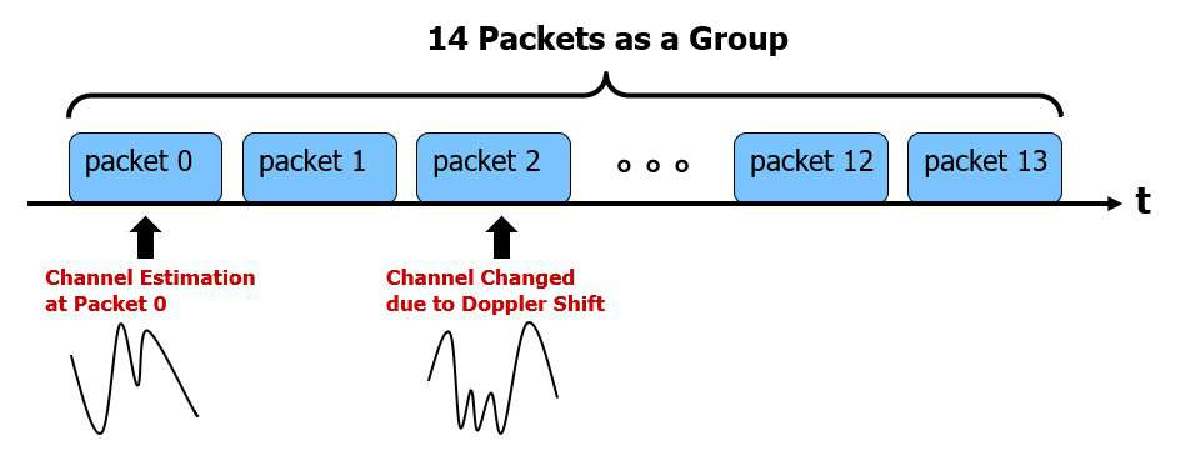
\includegraphics[width=\linewidth,clip]{fig/rayleigh_group.pdf}
		\caption{Illustration of Rayleigh Fading Channel}
		\label{fig:sample}
	\end{center}
\end{figure}

\begin{figure}[tbp]
	\begin{center}
		\vspace{0cm}
		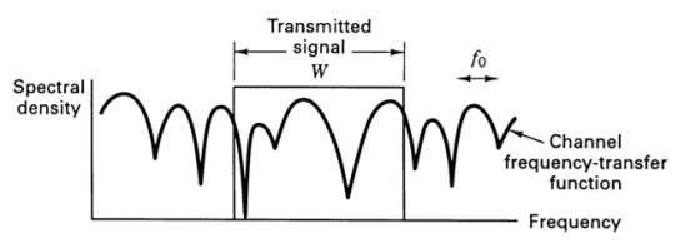
\includegraphics[width=\linewidth,clip]{fig/select_fading_illustrate.pdf}
		\caption{Illustration of Frequency Selective Fading Channel}
		\label{fig:sample}
	\end{center}
\end{figure}

\begin{table}[hb]
	\begin{center}
	\caption{SIMULATION CONDITIONS}
	\label{tbl:simu}
	\small
	\begin{tabular}{ll}
	\hline
	ITEMS & CONDITIONS\\
	\hline
	Moduation Method & QPSK/DQPSK \\
	Transmission Bits & 128 \\
	Group Size & 14 \\
	Channel & Rayleigh Fading/Selective Fading Channel \\
	Detection & Noncoherent/Coherent Detection \\
	Number of Trials & $10^{4}$ \\
	Decision Method & MLE \\
	Channel Estimation & $\hat{h}=h$ \\
	\hline
	\end{tabular}
	\end{center}
\end{table}

\begin{figure}[tbp]
	\begin{center}
		\vspace{0cm}
		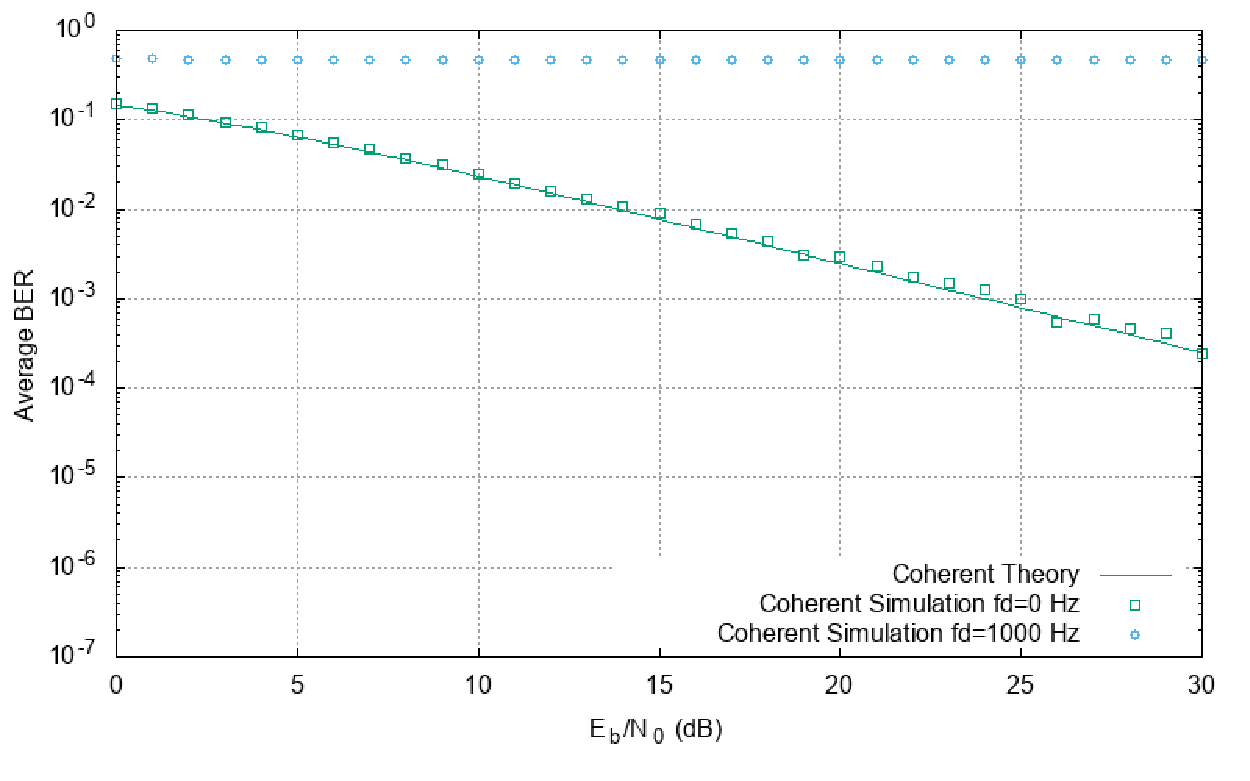
\includegraphics[width=\linewidth,clip]{fig/r_coherent.pdf}
		\caption{Coherent Demodulation BER with and without Phase Shift in Rayleigh Fading Channel}
		\label{fig:sample}
	\end{center}
\end{figure}

\begin{figure}[tbp]
	\begin{center}
		\vspace{0cm}
		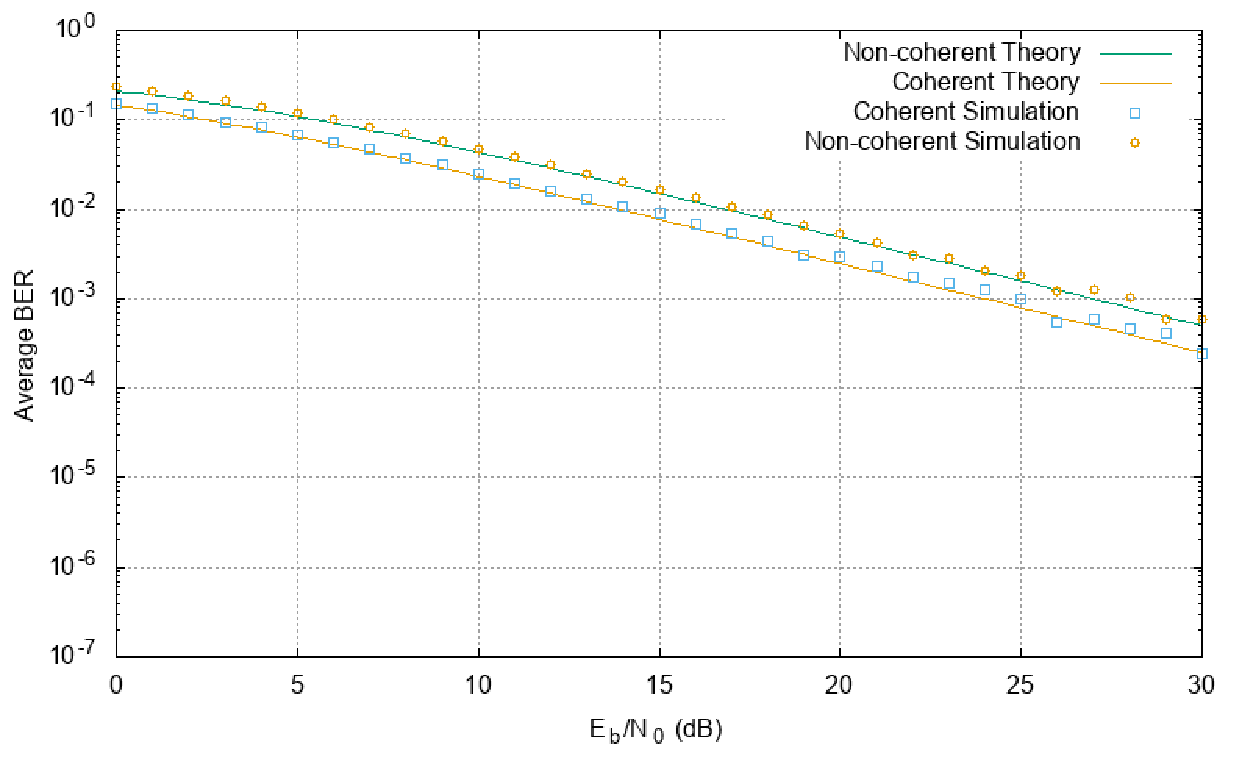
\includegraphics[width=\linewidth,clip]{fig/without_fd.pdf}
		\caption{Theoretic and Simulation BER without Doppler Shift in Rayleigh Fading Channel}
		\label{fig:sample}
	\end{center}
\end{figure}

\begin{figure}[tbp]
	\begin{center}
		\vspace{0cm}
		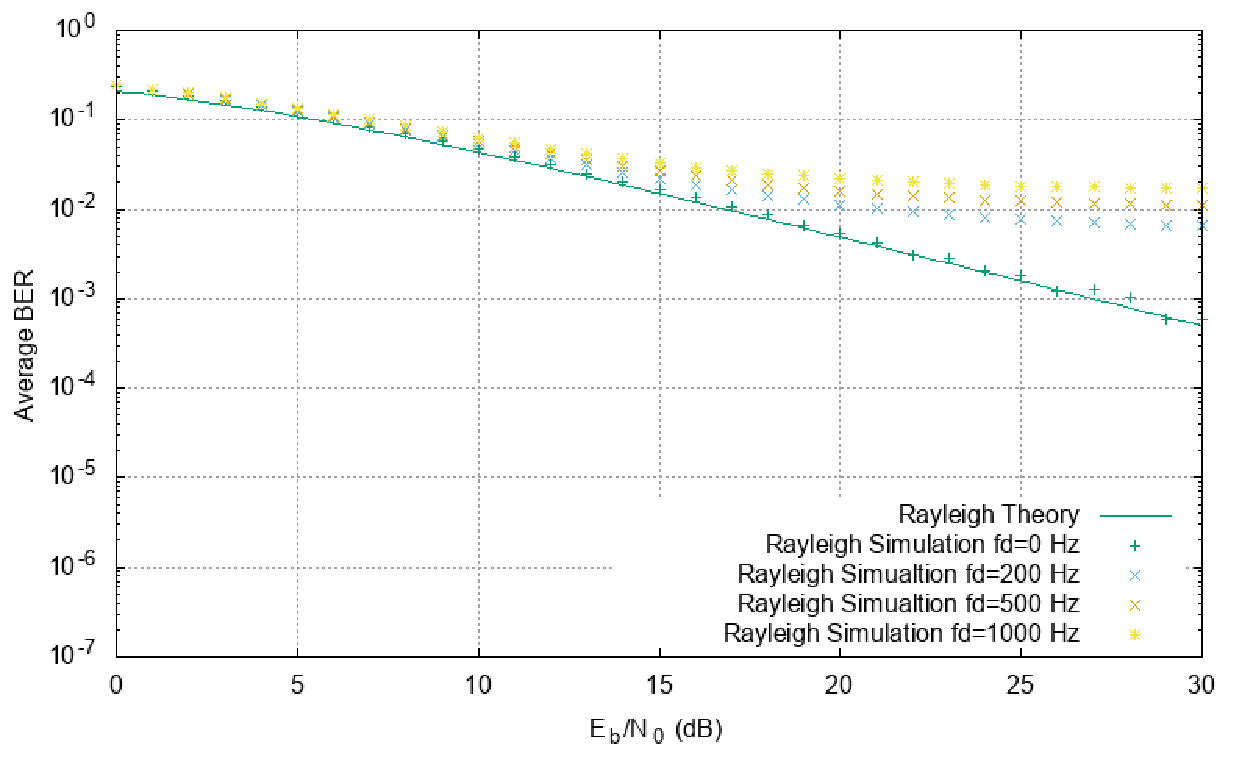
\includegraphics[width=\linewidth,clip]{fig/with_fd.pdf}
		\caption{QPSK and Noncoherent Demodulation BER with Different Doppler Shift in Rayleigh Fading Channel}
		\label{fig:sample}
	\end{center}
\end{figure}

\begin{figure}[tbp]
	\begin{center}
		\vspace{0cm}
		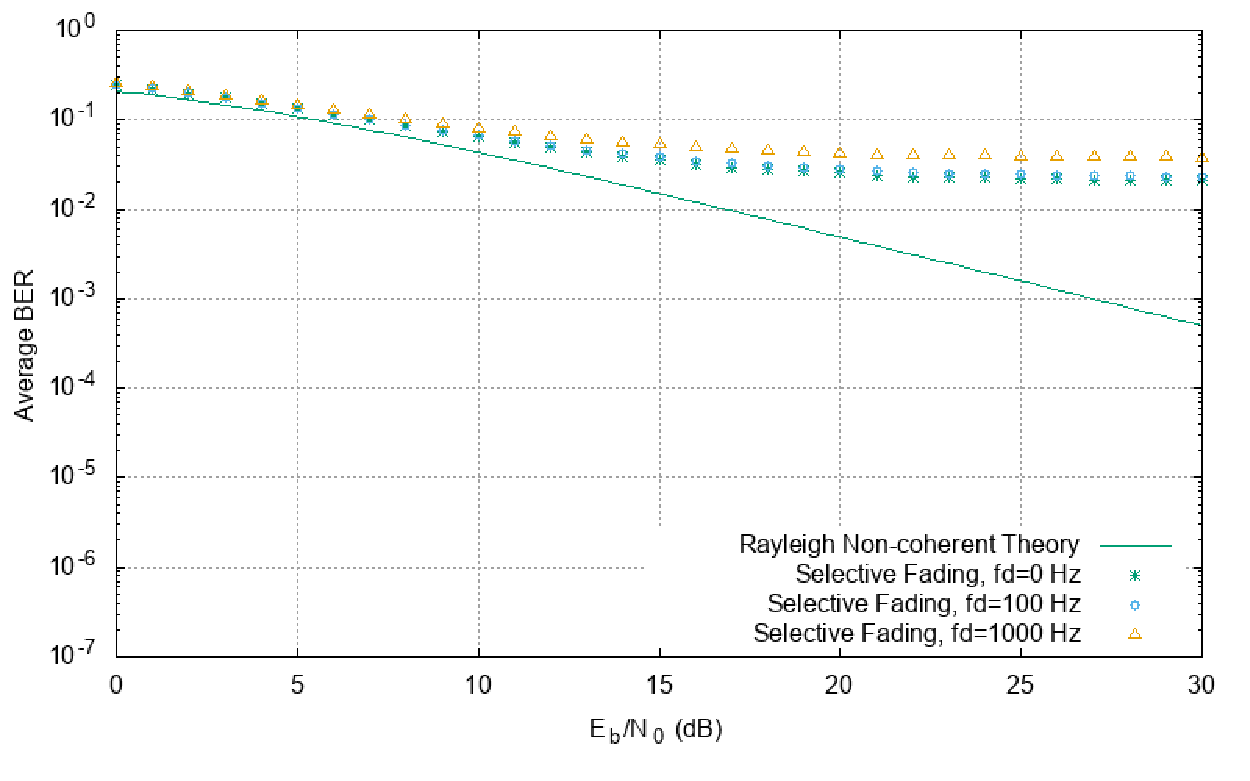
\includegraphics[width=\linewidth,clip]{fig/select.pdf}
		\caption{QPSK and Noncoherent Demodulation BER with Different Doppler Shift in Selective Fading Channel}
		\label{fig:sample}
	\end{center}
\end{figure}

\section{Simulation Result and Conclusion}

\bibliographystyle{IEEEtran}
\bibliography{rayleigh.bib}

\end{document} 